% !TeX spellcheck = da_DK
\section{Gangfunktion}
Knæet er et af kroppens vigtigste led for, at mennesket er i stand til at gå. Ved gang anvendes foruden knæleddet, hofte- og ankelleddet. Det er dog knæleddet, der står for den primære opgave ved udførelse af aktiviteter som at gå, løbe, og ved udførelse af øvelser som f.eks. squat. 

\subsection{Knæets opbygning}
Knæleddet er et hængselled, hvilket medvirker til at knæet kan udføre fleksion, ekstension og meget begrænset rotation. Knæet består af tre separate ledforbindelser. To der er forbundet mellem femur og tibia samt et mellem patella og petallas overflade af femur, hvilket fremgår af \ref{fig:knae_anatomi}. Ud over de tre separate ledforbindelser stabiliseres knæet af syv ledbånd. Senen som er ansvarlig under extension af knæet. Derudover er der to poplaterale ledbånd som strækker sig mellem femur, tibia og fibia, hvilket er med til at styrke knæleddets overflade posterior. Inde i ledkapslen befinder det forreste korsbånd (ACL) og det bagerste korsbånd (PCL), som har til opgave at fastgøre indre knoglefremspring af tibia til knoglefremspringet på femur. Korsbåndene har til opgave at begrænse anteriore og posterioe bevægelse af femur og er med til opretholdelse af retningen af knoglefremspringene. Det tibiale kollaterale ligament forstærker den mediale flade af knæleddet og fibular kollaterale ligament forstærker sidefladen, disse ligamenter anvendes kun ved fuld ekstension. 

\begin{figure}
\centering
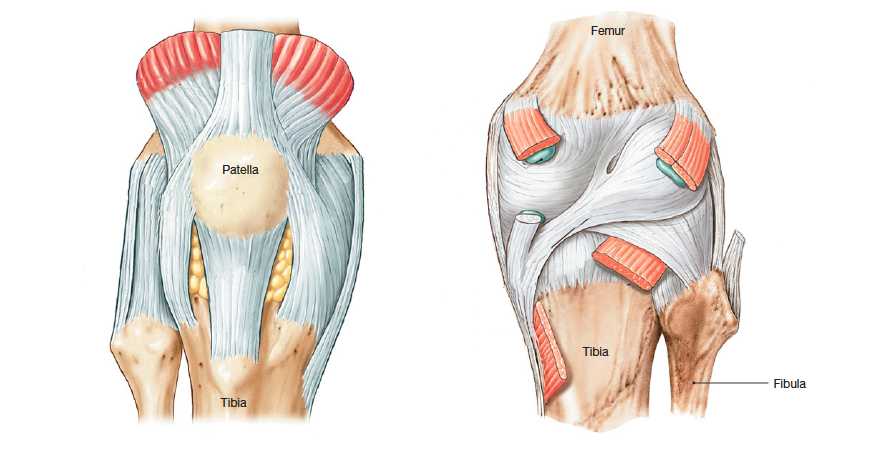
\includegraphics[width=0.45\textwidth]{figures/knae_anatomi}
\caption{På figuren ses knæets anatomiske opbygning}%\citep{kilde}
\label{fig:knae_anatomi}
\end{figure} 

\subsection{Knæets funktion}
Ved gang aktiveres quadriceps musklerne, der sidder anteriort på femur, og hamstring musklerne, der sidder poseriort på femur, hvilket fremgår af \ref{fig:knae_anatomi}. Quadriceps musklerne består af rectus femoris, vastus intermedius, vastus medialis og vastus lateralis. Hamstring musklerne består af biceps femoris, semitendinosus og semimembranosus. Ved bevægelse foretager quadriceps eller hamstring musklerne ekstension eller fleksion, hvorved de fungerer som hinandens agonist eller antagonist under bevægelse. 

Som tidligere nævnt er coxa, knæ og ankel de væsentligste faktorer der benyttes under gang. Udover selve holdningen er der også fokus på sving af leddene. Det fremgår af \ref{fig:knaet}, hvordan de forskellige led udfører fleksion, ekstension og går fra ekstension til neutral bevægelse under gang. 

\begin{figure}
\centering
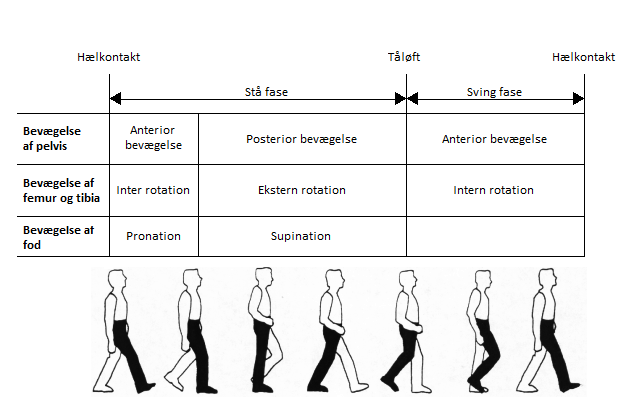
\includegraphics[width=1\textwidth]{figures/knaet}
\label{fig:knaet}
\caption{På figuren ses ekstension og fleksion af coxa, knæet og ankel ved gang}
\end{figure} 

\subsubsection{Knæet funktion under squat øvelse}
En af de øvelser hvor knæets er mest udsat er ved bøjning af knæet ved udførelse af en squat øvelse. Under denne øvelse aktiveres quadricepsmusklerne ved en 80-90 graders fleksion og er herefter konsistent, der ses en større aktivering af vastus intermedius, vastus medialis samt vastus lateris, da disse muskler er én ledmuskel, hvor rectus femoris er en to ledsmuskel. Hamstringmusklerne aktiveres ved en 45 graders fleksion. Dette er dog kun hvis øvelsen foretages ved statisk bevægelse.




 %der er forbundet mellem femur, tibia og patella. Knæet har fire ledbånd. To af disse er side-ligamenterne, der sidder omkring knæleddet. De resterende to er korsbåndene, der sidder på skrå inden i knæet.
%Knæet fire ledbånd sikrer stabilisering af knæet og sørger for at knoglerne bevæger sig rigtigt.  Det er knæleddet, der gør det muligt for kroppen at kunne udføre aktiviteter som at kunne gå, løbe, og eksempelvis squatte. Ved gang aktiveres både quadriceps musklerne (rectus femoris, vastus intermedius, vastus medialis, vastus lateralis) der sidder anteriort for låret samt hamstring musklerne (biceps femoris, semitendinosus, Semimembranosus), der sidder posteriort for låret og kontraherer med quadriceps musklerne. 

